\documentclass[12pt]{article}
\linespread{1.3}
\usepackage{hyperref}
\usepackage{enumitem}
%\usepackage{enumerate}
\usepackage{changepage,lipsum,titlesec, longtable}
\usepackage{cite}
\usepackage{comment, xcolor}
\usepackage[pdftex]{graphicx}
  \graphicspath{{images/}, {images/stat/}}
  \DeclareGraphicsExtensions{.pdf,.jpeg,.png, .jpg}
\usepackage[cmex10]{amsmath}
\usepackage{tikz}
\usepackage{array} 
\usepackage{subfigure} 
\newcommand{\grey}[1]{\textcolor{black!30}{#1}}
\newcommand{\red}[1]{\textcolor{red!50}{#1}}
\newcommand{\question}[1]{\textcolor{magenta}{\textbf{Question: } {#1}}}
\newcommand{\fref}[1]{Figure~\ref{#1}}
\newcommand{\tref}[1]{Table~\ref{#1}}
\newcommand{\eref}[1]{Equation~\ref{#1}}
\newcommand{\cref}[1]{Chapter~\ref{#1}}
\newcommand{\sref}[1]{Section~\ref{#1}}
\newcommand{\aref}[1]{Appendix~\ref{#1}}

\renewcommand{\labelenumii}{\theenumii}
\renewcommand{\theenumii}{\theenumi.\\arabic{enumii}.}

\oddsidemargin0cm
\topmargin-2cm %I recommend adding these three lines to increase the
\textwidth16.5cm %amount of usable space on the page (and save trees)
\textheight23.5cm

\makeatletter
\renewcommand\paragraph{\@startsection{paragraph}{4}{\z@}%
            {-2.5ex\@plus -1ex \@minus -.25ex}%
            {1.25ex \@plus .25ex}%
            {\normalfont\normalsize\bfseries}}
\makeatother
\setcounter{secnumdepth}{4} % how many sectioning levels to assign numbers to
\setcounter{tocdepth}{4}    % how many sectioning levels to show in ToC

% draw diagram
\usetikzlibrary{shapes.geometric, arrows}
\tikzstyle{data} = [font=\scriptsize, rectangle, rounded corners, minimum width=1.5cm, minimum height=1cm,align=left, draw=black, fill=black!30]
\tikzstyle{database} = [font=\scriptsize, rectangle, rounded corners, minimum width=3cm, minimum height=1cm,align=left, draw=black, fill=green!30]
\tikzstyle{query} = [font=\scriptsize,trapezium, trapezium left angle=70, trapezium right angle=110, minimum width=0.5cm, minimum height=0.5cm, text centered, draw=black, fill=blue!30]
\tikzstyle{process} = [font=\scriptsize,rectangle, minimum width=3cm, minimum height=1cm, text centered, draw=black, fill=orange!30]
\tikzstyle{spliter} = [font=\scriptsize,diamond, minimum width=2cm, minimum height=1cm, text centered, draw=black, fill=green!30]
\tikzstyle{decision} = [font=\scriptsize,diamond, minimum width=3cm, minimum height=1cm, text centered, draw=black, fill=green!30]
\tikzstyle{arrow} = [thick,->,>=stealth]
\tikzstyle{bi-arrow} = [thick,->,>=stealth]


\begin{document}
\title{Retrieving Building Snapshot ID\\
       \large SEED project}
\maketitle
\tableofcontents
\newpage
\section{Introduction}\label{sec:intro}
The document records the implementation of the PM template file
converter with the following main tasks:
\begin{itemize}
\item Converting legacy excel files downloaded from EnergyStar PM
  website to the proposed excel template.
\item Reading a folder containing the excel files with the template.
\item Uploading PM files to SEED (optional)
\item Querying SEED database to retrieve buildingsnapshot\_id and
  cononical\_building id
\item Converting template data to the json data format
\end{itemize}

\section{Flow Diagram with PM excel template}\label{sec:outline}
\subsection{Excel template}
The excel template consists of the following fields:
\begin{description}
\item[Street Address] corresponding to the "Address Line 1" in BEDES,
  "This address represents a complete street address, including street
  number, street name, prefixes, suffixes, modifiers, and unit
  number."\url{https://bedes.lbl.gov/bedes-online/address-line-1}
\item[Project Name] the name of the building, corresponding to the
  ``Name'' (Name identifying the premises. This could be the name of
  the complex, the building, or the space within a building, such as a
  classroom number) or ``Project'' (Identifier used to specify a
  certain
  project.)\url{https://bedes.lbl.gov/bedes-online/identifier-label}
\item[Portfolio Manager ID] corresponding to the ``Portfolio Manager
  Property'' in BEDES (``A unique ID assigned by EPA's Portfolio
  Manager program to each property. This is a unique ID assigned by
  EPA to each premises. A premises can be a portion of a building, a
  single building, or a campus of buildings. If the property is a
  campus of buildings and each building is benchmarked, individual
  buildings will also be assigned individual IDs, and the ID for the
  campus is referred to as the Parent Property
  ID.'').\url{https://bedes.lbl.gov/bedes-online/identifier-label}
  
  Note, this field is not be available for energy records for
  buildings that haven't been created in EnergyStar Portfolio
  Manager. It is used for holding the information from existing raw PM
  tables downloaded from EnergyStar. It can be used as a key field for
  searching SEED database and retrieving buildingsnapshot\_id
\item[Portfolio Manager Meter ID] corresponding to the ``Meter'' field
  in BEDES (``Identifier containing relevant meter
  information'')\url{https://bedes.lbl.gov/bedes-online/identifier-label}
\item[Meter Type] Corresponding to the field of ``Resource'' in BEDES
  (``Type of energy resource fuel. This can be applied at the premises
  or individual system or equipment
  level.'')\url{https://bedes.lbl.gov/bedes-online/resource}
\item[Start Date] Corresponding to the field of ``Interval Start
  Date'' in BEDES (``The start date that marks the beginning of the
  time interval for a value. Format for the date can be found in
  Metadata's "Date
  Format'')\url{https://bedes.lbl.gov/bedes-online/interval-start-date}
\item[End Date] Corresponding to the field of ``Interval End Date'' in
  BEDES (``The end date that marks the ending of the time interval for
  a value. Format for the date can be found in Metadata's "Date
  Format'')\url{https://bedes.lbl.gov/bedes-online/interval-end-date}
\item[Usage/Quantity] Corresponding to the field of ``Power Metric
  Value'' in BEDES (``Value of the measurement of associated power
  metric'')\url{https://bedes.lbl.gov/bedes-online/power-metric-value}
\item[Usage Units] Corresponding to ``Unit Of Measure'' in BEDES
  (``Unit of measurement for the data
  value.'')\url{https://bedes.lbl.gov/bedes-online/unit-measure}
\item[Cost] Corresponding to the field of ``Cost'' in BEDES (``Cost to
  related the project or measure. Must be associated with "Cost
  Attribution" and "Interval Period", if necessary.'')
\end{description}

\begin{figure}[h!]
  \centering
  \includegraphics[width = 1.0\textwidth]{template10field.png}
  \caption{Template excel file}
  \label{fig:template10field}
\end{figure}

\subsection{Pseudo Code}
\makeatletter
\def\verbatim@font{\linespread{1}\small\ttfamily}
\begin{verbatim}
User:
Fill out the PM template table with their building information
Upload tables to SEED database (making sure there is an ID created)
//Note: this step can be omitted, if the SEED platform provide some internal 
//place to hold the table so that we can download from this internal folder.
Upload tables to some remote folder (for us to download)

We:
Download the remote folder that contains the tables with the specified format.
For each table in the folder:
    Read the table into a data frame (Python pandas dataframe)
    //note: If the table is not uploaded to EnergyStar PM, 
    //the Portfolio Manager ID might not be available,
    //for tables converted from PM raw table, these fields are available
    //the assumption: each address uniquely identifies a building
    Get a set (dictionary key), A, of addresses from the PM table
    Create an empty dictionary D (initializing all entries to None)
        for each address a in the set A:
            make a QUERY to SEED database with address, 
                if address identifies a building b is in SEED database
                    //SEED.BuildingSnapshot.id
                    get the building snapshot id: s_id
                    make a QUERY with s_id to get c_id
                    //SEED.BuildingSnapshot.canonical_building
                    D[a] = {buildingsnapshot_id: s_id,
                            canonical_building: c_id}
                else 
                    D[a] = None
    Insert the c_id, s_id to the dataframe
    convert the dataframe to json format
\end{verbatim}
\subsubsection{Diagram}
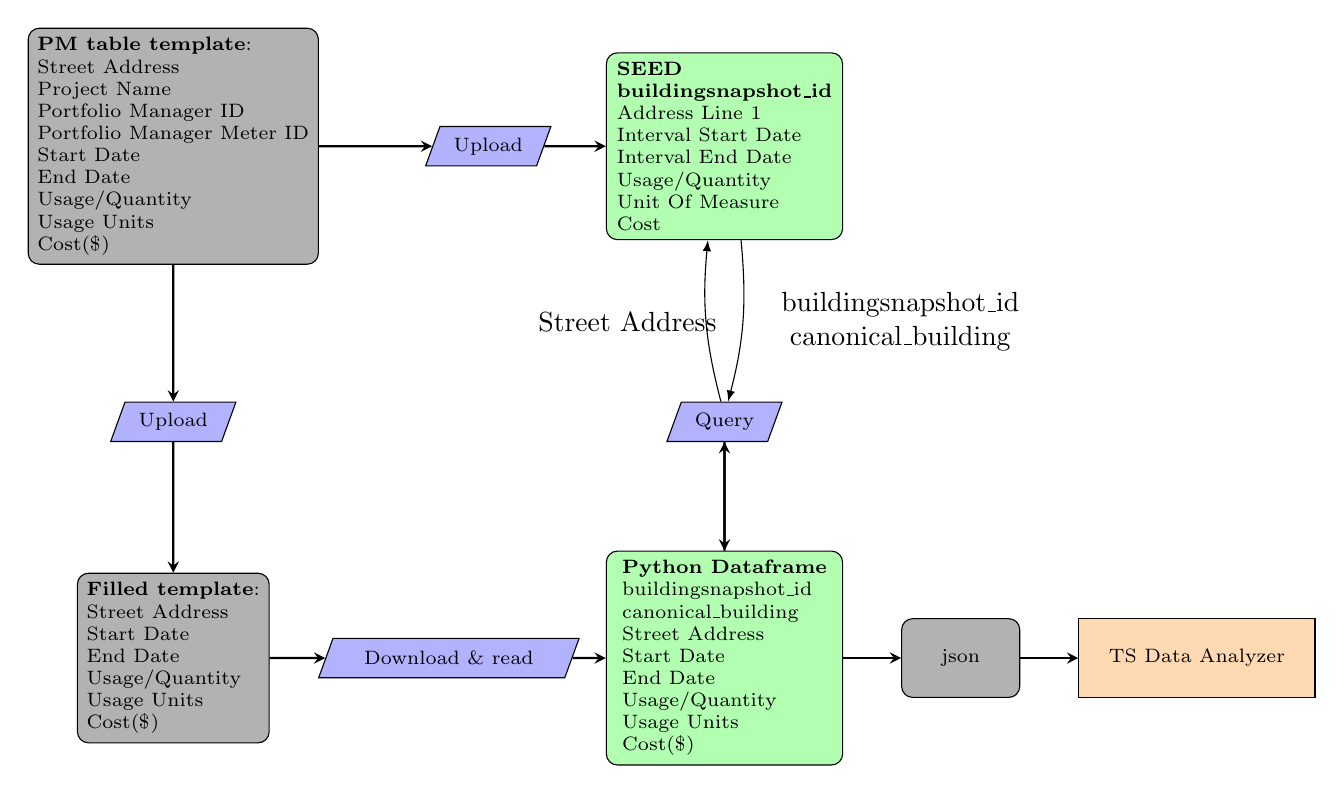
\begin{tikzpicture}
  \node (PM_table) [data]{\textbf{PM table template}:\\
    Street Address\\
    Project Name\\
    Portfolio Manager ID\\
    Portfolio Manager Meter ID\\
    Start Date\\
    End Date\\
    Usage/Quantity\\
    Usage Units\\
    Cost(\$)};
  \node (upload)[query, right of = PM_table, xshift=3cm]{Upload};
  \node (upload2)[query, below of = PM_table, yshift=-2.5cm]{Upload};
  \node (SEED db)[database, right of = upload, xshift=2cm]{\textbf{SEED}\\
    \textbf{buildingsnapshot\_id}\\
    Address Line 1\\
    Interval Start Date\\
    Interval End Date\\
    Usage/Quantity\\
    Unit Of Measure\\
    Cost};
  \node (remote folder) [data, below of=upload2, yshift=-2cm]{\textbf{Filled template}:\\
    Street Address\\
    Start Date\\
    End Date\\
    Usage/Quantity\\
    Usage Units\\
    Cost(\$)};
  \node (download)[query, right of = remote folder, xshift=2.5cm]{Download \& read};
  \node(dataframe)[database, right of=download, xshift = 2.5cm]{\textbf{Python Dataframe}\\
    buildingsnapshot\_id\\
    canonical\_building \\
    Street Address\\
    Start Date\\
    End Date\\
    Usage/Quantity\\
    Usage Units\\
    Cost(\$)};
  \node(query)[query, above of=dataframe, yshift=2cm]{Query};
  \node(json)[data, right of=dataframe, xshift=2cm]{json};
  \node(ext)[process, right of=json, xshift=2cm]{TS Data Analyzer};
  \draw[arrow](PM_table) -- (upload);
  \draw[arrow](upload) -- (SEED db);
  \draw[arrow](PM_table) -- (upload2);
  \draw[arrow](upload2) -- (remote folder);
  \draw[arrow](remote folder) -- (download);
  \draw[arrow](download) -- (dataframe);
  \draw[arrow](dataframe) -- (query);
  \draw[arrow](query) -- (dataframe);
  \draw[arrow](dataframe) -- (json);
  \draw[arrow](json) -- (ext);
  \draw[-latex] (query) to[bend left=10] node [xshift=-1cm]{Street Address} (SEED
  db); 
  \draw[-latex] (SEED db) to[bend left=10] node [xshift=2cm,align=center]{buildingsnapshot\_id\\canonical\_building}
  (query);
\end{tikzpicture}

\subsection{Retrieving Building Snapshot ID}
Wrote a query.py file to query SEED test database and retrieve 
\section{PM Excel file to template file converter}
Wrote a PM2template.py file to convert EnergyStar PM file to the excel
template
\section{Modified flow chart}

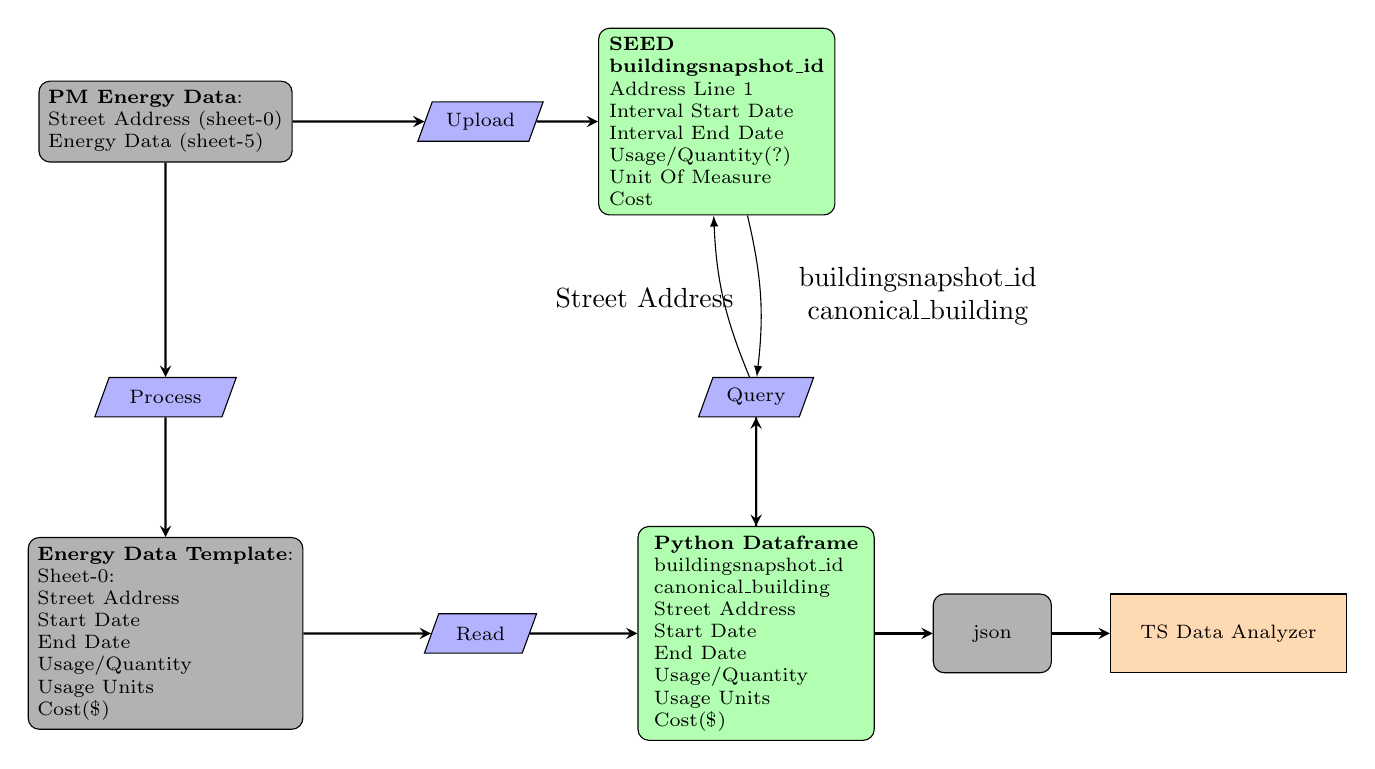
\begin{tikzpicture}
  \node (PM_table) [data]{\textbf{PM Energy Data}:\\
    Street Address (sheet-0)\\
    Energy Data (sheet-5)};
  \node (upload)[query, right of = PM_table, xshift=3cm]{Upload};
  \node (upload2)[query, below of = PM_table, yshift=-2.5cm]{Process};
  \node (SEED db)[database, right of = upload, xshift=2cm]{\textbf{SEED}\\
    \textbf{buildingsnapshot\_id}\\
    Address Line 1\\
    Interval Start Date\\
    Interval End Date\\
    Usage/Quantity(?)\\
    Unit Of Measure\\
    Cost};
  \node (remote folder) [data, below of=upload2, yshift=-2cm]{\textbf{Energy Data Template}:\\
    Sheet-0:\\
    Street Address\\
    Start Date\\
    End Date\\
    Usage/Quantity\\
    Usage Units\\
    Cost(\$)};
  \node (download)[query, right of = remote folder, xshift=3cm]{Read};
  \node(dataframe)[database, right of=download, xshift = 2.5cm]{\textbf{Python Dataframe}\\
    buildingsnapshot\_id\\
    canonical\_building \\
    Street Address\\
    Start Date\\
    End Date\\
    Usage/Quantity\\
    Usage Units\\
    Cost(\$)};
  \node(query)[query, above of=dataframe, yshift=2cm]{Query};
  \node(json)[data, right of=dataframe, xshift=2cm]{json};
  \node(ext)[process, right of=json, xshift=2cm]{TS Data Analyzer};
  \draw[arrow](PM_table) -- (upload);
  \draw[arrow](upload) -- (SEED db);
  \draw[arrow](PM_table) -- (upload2);
  \draw[arrow](upload2) -- (remote folder);
  \draw[arrow](remote folder) -- (download);
  \draw[arrow](download) -- (dataframe);
  \draw[arrow](dataframe) -- (query);
  \draw[arrow](query) -- (dataframe);
  \draw[arrow](dataframe) -- (json);
  \draw[arrow](json) -- (ext);
  \draw[-latex] (query) to[bend left=10] node [xshift=-1cm]{Street Address} (SEED
  db); 
  \draw[-latex] (SEED db) to[bend left=10] node [xshift=2cm,align=center]{buildingsnapshot\_id\\canonical\_building}
  (query);
\end{tikzpicture}
\newpage
\bibliographystyle{plain}
\bibliography{myCitation}
\end{document}